\documentclass[12pt, titlepage]{article}
\usepackage[normalem]{ulem}
\usepackage{fullpage}
\usepackage[round]{natbib}
\usepackage{multirow}
\usepackage{booktabs}
\usepackage{tabularx}
\usepackage{graphicx}
\usepackage{float}
\usepackage{hyperref}
\hypersetup{
    colorlinks,
    citecolor=black,
    filecolor=black,
    linkcolor=red,
    urlcolor=blue
}
\usepackage[round]{natbib}

\newcounter{acnum}
\newcommand{\actheacnum}{AC\theacnum}
\newcommand{\acref}[1]{AC\ref{#1}}

\newcounter{ucnum}
\newcommand{\uctheucnum}{UC\theucnum}
\newcommand{\uref}[1]{UC\ref{#1}}

\newcounter{mnum}
\newcommand{\mthemnum}{M\themnum}
\newcommand{\mref}[1]{M\ref{#1}}

\newcounter{fnum}
\newcommand{\fthefnum}{R\thefnum}
\newcommand{\fref}[1]{R\ref{#1}}

\title{SE 3XA3: Module Guide\\Spaceshooter Remix}

\author{Team \#4, IRS Development
        \\ Ibrahim Malik maliki2
        \\ Ryan Schnekenburger schneker
        \\ Saad Khan khans126
}

\date{\today}

\begin{document}

\maketitle

\pagenumbering{roman}
\tableofcontents
\listoftables
\listoffigures

\newpage

\begin{table}[hp]
\caption{Revision History} \label{TblRevisionHistory}
\begin{tabularx}{\textwidth}{llX}
\toprule {\bf Date} & {\bf Version} & {\bf Notes}\\
\midrule
5 November 2018 & Rev 0 & Authored by Ibrahim, Saad, Ryan\\
December 5, 2018 & Rev1 & Updated document and added the changes recommended by TA.\\
\bottomrule
\end{tabularx}
\end{table}

\newpage

\pagenumbering{arabic}

\section{Introduction}

\subsection{Overview}
The project is re-implementation of the classic space shooter game that was popular in the 1980s and 1990s. There are several versions of this game online, but we attempt to create it for a computer using Python 3. This game will require a keyboard and will hopefully provide a retro feel to the user which will create a nostalgic effect. The objective of the game is to survive for as long as possible by destroying or avoiding the asteroids.

\subsection{Context}
There are 2 specific documents in this design and document specification. This document is the Module Guide (MG) and there is also Module Interface Specification (MIS) document. 
\\
\newline The Module Guide was based on the original Software Requirements Specification (SRS) which outlined exactly the purpose and the main objectives of this project. There were several functional and non-functional requirements that were outlined in that document that detailed the expectations for the game. This document will provide a modular decomposition of the implementation of the system. It will show how this game can be executed to meet both functional and nonfunctional requirements. It will display the architectural design of this system describing the modules, the rationale for decomposition, the relationship between the modules and any constraints that will need to be respected. 
\\
\newline The MIS document is based off the Module Guide. It will describe the semantics of each module and include assumptions, state variables, environment variables, uses, access routines, and exceptions. Every function or method will be described in this manner showing the inputs and outputs and provide a basis of how each module is executed. It is an example of a detailed design. 
\\ 
\newline Decomposing a system into modules is a commonly accepted approach to developing
software.  A module is a work assignment for a programmer or programming
team~\citep{ParnasEtAl1984}.  We advocate a decomposition
based on the principle of information hiding~\citep{Parnas1972a}.  This
principle supports design for change because the ``secrets'' that each module
hides represent likely future changes.  Design for change is valuable in SC,
where modifications are frequent, especially during initial development as the
solution space is explored.  
\\
\newline Our design follows the rules laid out by \citet{ParnasEtAl1984}, as follows:

\begin{itemize}
\item System details that are likely to change independently should be the
  secrets of separate modules.
\item Each data structure is used in only one module.
\item Any other program that requires information stored in a module's data
  structures must obtain it by calling access programs belonging to that module.
\end{itemize}

This document will be helpful for the following people:

\begin{itemize}
\item New project members: This document can be a guide for a new project member
  to easily understand the overall structure and quickly find the relevant modules they are searching for.
\item Maintainers: The hierarchical structure of the module guide improves the
  maintainers' understanding when they need to make changes to the system. It is important for a maintainer to update the relevant sections of the document after changes have been made.
\item Designers: Once the module guide has been written, it can be used to
  check for consistency, feasibility, and flexibility. Designers can verify the system in various ways, such as consistency among modules, the feasibility of the decomposition, and flexibility of the design.
\end{itemize}

\subsection{Design Principles}


\subsection{Document Structure}
The document is organized as below:
\begin{itemize}
\item \ref{SecChange} will list the unlikely and anticipated changes of the software requirements. 
\item Section \ref{SecMH} will summarize the module decomposition and present a hierarchy separating different decision modules
\item Section \ref{SecConnection}
specifies the connections between the software requirements and the
modules. 
\item Section \ref{SecMD} gives a detailed description of the
modules. 
\item Section \ref{SecTM} includes two traceability matrices. One checks
the completeness of the design against the requirements provided in the SRS. The
other shows the relation between anticipated changes and the modules.
\item Section \ref{SecUse} demonstrates how the modules are connected to each other.
\end{itemize}

\section{Anticipated and Unlikely Changes} \label{SecChange}

This section lists possible changes to the system. The possible changes are classified into two
categories according to the likeliness of change. Anticipated changes are listed in Section \ref{SecAchange}, and
unlikely changes are listed below that in Section \ref{SecUchange}.

\subsection{Anticipated Changes} \label{SecAchange}

Anticipated changes refer to the source of information that is within the modules and how changing that will affect the system. Changing one of the anticipated changes will require only one module being changed that will hide the associated decision. This allows for versatility for change without majorly impacting the rest of the project and is called design for change.

\begin{description}
\item[\refstepcounter{acnum} \actheacnum \label{acHardware}:] The 
  hardware or computer on which the software is running.
\item[\refstepcounter{acnum} \actheacnum \label{acAlg}:] Algorithms for controlling the speed, power or the movement of the sprites
\item[\refstepcounter{acnum} \actheacnum \label{acObjects}:] The images of the game objects can be changed. This includes game objects like characters and asteroids. There will likely be an increase in the number of objects. 
\item[\refstepcounter{acnum} \actheacnum \label{acPlay}:] There will be a change in the gameplay to allow for increased difficulty of the gameplay as game time progresses 
\item[\refstepcounter{acnum} \actheacnum \label{acMenu}:] Additional menus providing instructions or credits is likely

\end{description}

\subsection{Unlikely Changes} \label{SecUchange}

The module design should be as general as possible. Nevertheless, a general system can be more complex. To avoid risking modification of several modules at once, these changes are unlikely. 

\begin{description}
\item[\refstepcounter{ucnum} \uctheucnum \label{ucIO}:] Input/Output devices
  (Input: Keyboard, Output: Screen).
\item[\refstepcounter{ucnum} \uctheucnum \label{ucInput}:] Input data will always come externally from the software
\item[\refstepcounter{ucnum} \uctheucnum \label{ucP3}:] The python 3 implementation of the game
\item[\refstepcounter{ucnum} \uctheucnum \label{ucPurpose}:] The purpose of the game and the objectives of destroying or avoiding asteroids

\end{description}

\section{Module Hierarchy} \label{SecMH}
This section provides an overview of the module design. Modules are summarized
in a hierarchy decomposed by secrets in Table \ref{TblMH}. The modules listed
below, which are leaves in the hierarchy tree, are the modules that will
actually be implemented.

\begin{description}
\item[\refstepcounter{mnum} \mthemnum \label{mHA}:] \sout{Player Module} 
\item[\refstepcounter{mnum} \mthemnum \label{mHB}:] Constants module
\item[\refstepcounter{mnum} \mthemnum \label{mHC}:] Spawn module
\item[\refstepcounter{mnum} \mthemnum \label{mHD}:] Asteroids module
\item[\refstepcounter{mnum} \mthemnum \label{mHE}:] Animations Module
\item[\refstepcounter{mnum} \mthemnum \label{mHF}:] Destroy module
\item[\refstepcounter{mnum} \mthemnum \label{mHG}:] IRS\_Space\_Shooter Module
\item[\refstepcounter{mnum} \mthemnum \label{mHH}:] Player\_Control
\item[\refstepcounter{mnum} \mthemnum \label{mHI}:] Player\_Hide
\item[\refstepcounter{mnum} \mthemnum \label{mHJ}:] Player\_Move
\item[\refstepcounter{mnum} \mthemnum \label{mHK}:] Player\_Shoot
\item[\refstepcounter{mnum} \mthemnum \label{mHL}:] Overheat\_Control
\end{description}

\begin{table}[h!]
\centering
\begin{tabular}{p{0.3\textwidth} p{0.6\textwidth}}
\toprule
\textbf{Level 1} & \textbf{Level 2}\\
\midrule

{Hardware-Hiding Module} & ~ \\
\midrule

\multirow{3}{0.3\textwidth}{Behaviour-Hiding Module} 
& Player\_Hide\\
& constants module\\
& Spawn module \\
& Asteroids module\\
& Player\_Move\\
\midrule

\multirow{2}{0.3\textwidth}{Software Decision Module} 
& Animations Module\\
& Destroy module\\
& IRS\_Space\_Shooter Module\\
& Overheat\_Control\\
& Player\_Control\\
& Player\_Shoot\\
\bottomrule

\end{tabular}
\caption{Module Hierarchy}
\label{TblMH}
\end{table}

\section{Connection Between Requirements and Design} \label{SecConnection}
The system is designed to satisfy the requirements that were outlined in the SRS. The system is decomposed to modules and the connections between requirements and modules are listed in Table \ref{TblRT}. The appearance and usability requirements will be satisfied with the input module which creates the initial environment to allow the user to interact within. That will be the game window. Then the requirements of the actual gameplay involving the movement of the players and the asteroids will be created by the Animations and IRS\_Space\_Shooter module. This module will also affect the precision, reliability, capacity and environmental requirements. The player, spawn and asteroid module will contribute to the appearance requirement as well. The game will be easy for the user to install because instructions will be given clearly and the user will just have to execute the game using a simple python command. Most computers have python compilers and this will satisfy the cross-platform ability of the game. All the commands and language used in the input and output modules will be clear and avoid any political or cultural violations. There is no data stored in any of the modules and hence no risk of private user information being a security risk. 

\section{Module Decomposition} \label{SecMD}


\subsection{Hardware Hiding Modules }


\subsection{Behaviour-Hiding Module}

\begin{description}
\item[Secrets:]Updating the sprite array, and calculating asteroid damage
\item[Services:] Constantly updates the sprite array when anything dies, and also deals damage to spaceship according to asteroid size
\item[Implemented By:] M7
\end{description}

\begin{description}
	\item[Secrets:]Visibility of the Player Sprite
	\item[Services:] Hides the player sprite upon death, and has it reappear once the game starts again
	\item[Implemented By:] M9
\end{description}

\begin{description}
	\item[Secrets:]Spawning sprites for missle and power ups
	\item[Services:] Adds sprites to groups that are drawn, when missles are shot or powerups are dropped
	\item[Implemented By:] M3	
\end{description}

\begin{description}
	\item[Secrets:]Decides movement speed of player
	\item[Services:] Adds values to the player movement parameters, allowing the player to move side to side
	\item[Implemented By:] M10
\end{description}




\subsubsection{Input Format Module}

\begin{description}
\item[Secrets:] Taking in sounds and images 
\item[Services:]Takes in images and sounds files and transforms them into useable forms 
\item[Implemented By:] M7
\end{description}



\subsection{Software Decision Module}

\begin{description}
\item[Secrets:] Displays all non-gameplay sprites
\item[Services:] Draws all sprites such as lives, health, and menu

\item[Implemented By:] M5
\end{description}

\begin{description}
	\item[Secrets:] Deals with death animations
	\item[Services:] Once a sprite dies, this module changes the image to an explosion and removes the sprite from the group
	
	\item[Implemented By:] M6
\end{description}

\begin{description}
	\item[Secrets:] Runs the Game
	\item[Services:] Runs the main game loop, and calls for updates for all sprites 
	\item[Implemented By:] M7
\end{description}

\begin{description}
	\item[Secrets:] Controls the overheat mechanic
	\item[Services:] Keeps track of how far along the player is on the overheat bar, and if the player overheats, doesnt allow the player to shoot 
	\item[Implemented By:] M12
\end{description}

\begin{description}
	\item[Secrets:] Player values
	\item[Services:] Keeps track of all player values, and send commands to other modules for updates.
	\item[Implemented By:] M8
\end{description}

\begin{description}
	\item[Secrets:] Controls shooting
	\item[Services:] Controls shooting for the player, and also sends updates to the overheat module to keep track of the overheat bar
	\item[Implemented By:] M12
\end{description}




\section{Traceability Matrix} \label{SecTM}

This section shows two traceability matrices: between the modules and the
requirements and between the modules and the anticipated changes.

% the table should use mref, the requirements should be named, use something
% like fref
\begin{table}[H]
\centering
\begin{tabular}{p{0.2\textwidth} p{0.6\textwidth}}
\toprule
\textbf{Req.} & \textbf{Modules}\\
\midrule
\fref{fRA} & \mref{mHF}\\
\fref{fRB} & \mref{mHF}, \mref{mHE}\\
\fref{fRC} & \mref{mHE}\\
\fref{fRD} & \mref{mHE}\\
\fref{fRE} & \mref{mHG}, \mref{mHC}\\
\fref{fRF} & \mref{mHG}\\
\fref{fRG} & \mref{mHF}\\
\fref{fRH} & \mref{mHG}\\
\fref{fRI} & \mref{mHA}\\
\fref{fRJ} & \mref{mHG}\\
\fref{fRK} & \mref{mHA}\\
\fref{fRL} & \mref{mHA}\\
\fref{fRM} & \mref{mHG}, \mref{mHE}\\
\fref{fRN} & \mref{mHA}\\
\bottomrule
\end{tabular}
\caption{Trace Between Requirements and Modules}
\label{TblRT}
\end{table}

\begin{table}[H]
\centering
\begin{tabular}{p{0.2\textwidth} p{0.6\textwidth}}
\toprule
\textbf{AC} & \textbf{Modules}\\
\midrule
\acref{acHardware} & \mref{mHG}\\
\acref{acAlg} & \mref{mHD}, \mref{mHA}, \mref{mHE}\\
\acref{acObjects} & \mref{mHD}, \mref{mHA}, \mref{mHC}\\
\acref{acPlay} & \mref{mHA}\\
\acref{acMenu} & \mref{mHE}, \mref{mHG}\\
\bottomrule
\end{tabular}
\caption{Trace Between Anticipated Changes and Modules}
\label{TblACT}
\end{table}

\section{Use Hierarchy Between Modules} \label{SecUse}

In this section we have a uses hierarchy wherein A will need B to execute but, B can execute without the use of A. The uses relation can been translated right from python by observing the import statement and where there exists an import statement that is a uses relation between that module and the import statement. Of course since we are creating a game each of our modules use pygame however I did not include that since it is a pre-created library. This is of the form of a directed acyclic graph (DAG) where you may start from any of the nodes and take a path but you will not be able to return to the node that you began on from each node.

\begin{figure}[H]
\centering
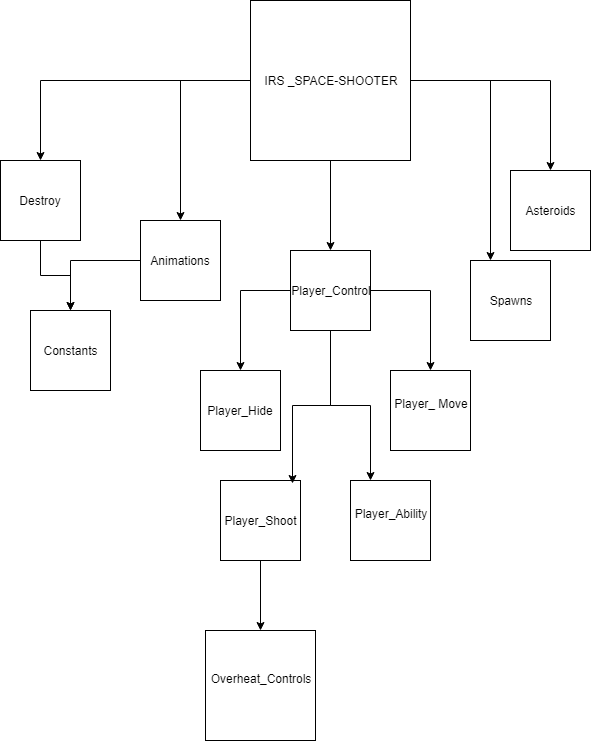
\includegraphics[width=0.7\textwidth]{pic1}
\caption{Use hierarchy among modules}
\label{FigUH}
\end{figure}

\section{Functional Requirements Reference} \label{SecFunc}

\begin{description}

\item [\refstepcounter{fnum} \fthefnum \label{fRA}:] 
When the game is executed in python a new window shall be opened
\\Fit Criterion or Test Case: Is a new window opened after the program is executed?

\item [\refstepcounter{fnum} \fthefnum \label{fRB}:] 
The game shall open a main menu once executed in python
\\Fit Criterion or Test Case: check to see if there is a main menu when you first execute the game

\item [\refstepcounter{fnum} \fthefnum \label{fRC}:] 
A loading screen will be displayed once 'enter' is pressed when the main menu is displayed
\\Fit Criterion or Test Case: press enter when on the main menu and see if a loading screen is displayed

\item [\refstepcounter{fnum} \fthefnum \label{fRD}:] 
Score shall increase when an asteroid comes in contact with a bullet
\\Fit Criterion or Test Case: check to see if the score increases when a bullet comes in contact with an asteroid on the game screen

\item [\refstepcounter{fnum} \fthefnum \label{fRE}:] 
Asteroids shall be removed from the game display once shot
\\Fit Criterion or Test Case: When in game and not in the main menu or the loading screen, check to see if when a bullet comes in contact with an asteroid that asteroid is no longer on the game screen

\item [\refstepcounter{fnum} \fthefnum \label{fRF}:] 
The health bar shall decrease if the ship comes in contact with an asteroid
\\Fit Criterion or Test Case: check to see if the health bar decreases once when hit by an asteroid on the game screen

\item [\refstepcounter{fnum} \fthefnum \label{fRG}:] 
The ship shall move to the left when the left arrow key is hit
\\Fit Criterion or Test Case: press the left arrow key and check if the ship moves left on the game screen

\item [\refstepcounter{fnum} \fthefnum \label{fRH}:] 
When the 'r' key is hit, all scores will be cleared
\\Fit Criterion or Test Case: Check that the score is 0 once the 'r' key is hit while on the game screen

\item [\refstepcounter{fnum} \fthefnum \label{fRI}:] 
When the spacebar is tapped one bullet is fired
\\Fit Criterion or Test Case: press the spacebar and check to see if a bullet is fired when on the game screen

\item [\refstepcounter{fnum} \fthefnum \label{fRJ}:] 
When the right arrow key is pressed the ship shall move to the right
\\Fit Criterion or Test Case: press the right arrow key and check if the ship moves to the right when on the game screen

\item [\refstepcounter{fnum} \fthefnum \label{fRK}:] 
When the 'q' button is pressed when the main menu is displayed the window shall close
\\Fit Criterion or Test Case: When the main menu is displayed press the q key and check to see if the window displaying the main menu is still open

\item [\refstepcounter{fnum} \fthefnum \label{fRL}:] 
When the health bar is empty a life is removed from the game screen
\\Fit Criterion or Test Case: Check to see if the amount of lives is one less than it was when the health bar was not empty on the game screen

\item [\refstepcounter{fnum} \fthefnum \label{fRM}:] 
When the player has no lives and their health bar is empty the main menu should be displayed
\\Fit Criterion or Test Case: Check to see if the main menu is displayed once the health bar is empty and there are no lives remaining on the game screen

\item [\refstepcounter{fnum} \fthefnum \label{fRN}:] 
When the health bar is zero the ship shall be temporarily removed from the screen
\\Fit Criterion or Test Case: Check to see if the ship is still displayed on the game screen when the health bar is empty

\end{description}

\newpage

%\section*{References}

\bibliographystyle {plainnat}
\bibliography {MG}

\end{document}